\documentclass[9pt]{beamer}
\usepackage{styles/mypreamble}
%~~~~~~~~~~~~~~~~~~~~~~~~~~~~~~~~~~~~~~~~~~~~~~~~~~~~~~~~~~~~~~~~~~~~~~~~~~~~~~
\title{Алгоритмы машинного обучения}
\subtitle{Лекция 7. Рекомендательные системы - 2}
\author{Владимир Кукушкин}
\institute{СПбГЭУ - 30.12.2020}
%~~~~~~~~~~~~~~~~~~~~~~~~~~~~~~~~~~~~~~~~~~~~~~~~~~~~~~~~~~~~~~~~~~~~~~~~~~~~~~

\begin{document}

\titlepage


\section{Content-based подход}

\begin{frame}{Предпосылки}
\begin{itemize}
    \item User-based и item-based подходы вполне рабочие, но но они используют только исторические оценки пользователей, но не используют никакую характерную информацию о пользователях объектах. Для начала это неплохо, но лучше расширить информативность данных.
    \item Хотелось бы строить портрет пользователей и объектов, и делать рекомендации в зависимости от этих данных.
\end{itemize}
\end{frame}

\framedgraphic{Пример карточки товара}{img/content_types.png}

\begin{frame}{Как это выглядит}
    \begin{itemize}
        \item Строим фичи для описания объектов. Для пользователей значения таких фичей будут отражать исторический выбор соответствующих объектов.
    \end{itemize}
    \begin{center}
        \begin{tabular}{c|c|c|c|c}
             & Комедия & Боевик & Вестерн & Триллер  \\ \hline
             фильм 1& 1 & 0 & 0 & 0 \\ \hline
             фильм 2& 1 & 0 & 0 & 1 \\\hline
             user 1& 0.3 & 0.1 & 0.2 & 0.4 \\\hline
             user 2& 0.1 & 0.2 & 0.3 & 0.4 \\
        \end{tabular}
    \end{center}
    \begin{itemize}
        \item Теперь пользователи и объекты находятся в одном фичовом пространстве, а значит можно находить ближайшие объекты для каждого пользователя и рекомендовать их.
        \item Метрика: обычно косинус.
    \end{itemize}
\end{frame}

\begin{frame}{Неструктурированные фичи}
    Ещё фичи бывают:
    \begin{itemize}
        \item Текстовые (аннотация, рецензия, и т.д.). Часто работает при холодном старте (когда нет информации об объекте), потому что с новым товаром обычно идёт хоть какое-то текстовое описание (рецензия).
        \item Изображения. Хорошо работает, например, в магазинах одежды. Рекомендуем одежду, похожую визуально на то, что пользователь покупал ранее.
    \end{itemize}
\end{frame}

\begin{frame}{Плюсы, минусы, подводные камни}
    \begin{itemize}
        \item Увеличили информативность данных, а значит есть надежда, что алгоритм на таких данных будет давать результат лучше, чем user/item-based подход.
        \item Много ручной работы. Информацию о всех объектах надо как-то вбить в базу. Иногда удаётся частично автоматизировать процесс, но всё равно поддерживать гору контента довольно непросто.
        \item Подпространство пользователей по-прежнему разрежено.
    \end{itemize}
\end{frame}

\section{Понижение размерности user-item матрицы}

\begin{frame}{Проблемы user-item представления}
Проблемы user-item представления
    \begin{itemize}
        \item Разреженность
        \item Оценки товаров часто коррелируют
    \end{itemize}
Q: Как бы эту матрицу хранить более компактно?\newline
A: Можно воспользоваться методами понижения размерности: PCA или SVD-разложение.
\end{frame}

\begin{frame}{SVD-разложение}
\begin{itemize}
    \item Разложим user-item матрицу: $R = U\Sigma V^T$. Количество главных компонент $k$ -- параметр.
    \item Для удобства переобозначим $U := U\Sigma$.
    \item Теперь все пользователи и все объекты помещены в одно и то же пространство размерности $k$.
    \item Пусть пользователю $u$ соответствует строка $p_u$ матрицы $U$, а объекту $i$ -- столбец $q_i$ матрицы $V$. Тогда $\hat r_{ui} = \langle p_u, q_i \rangle$.
\end{itemize}
\begin{center}
    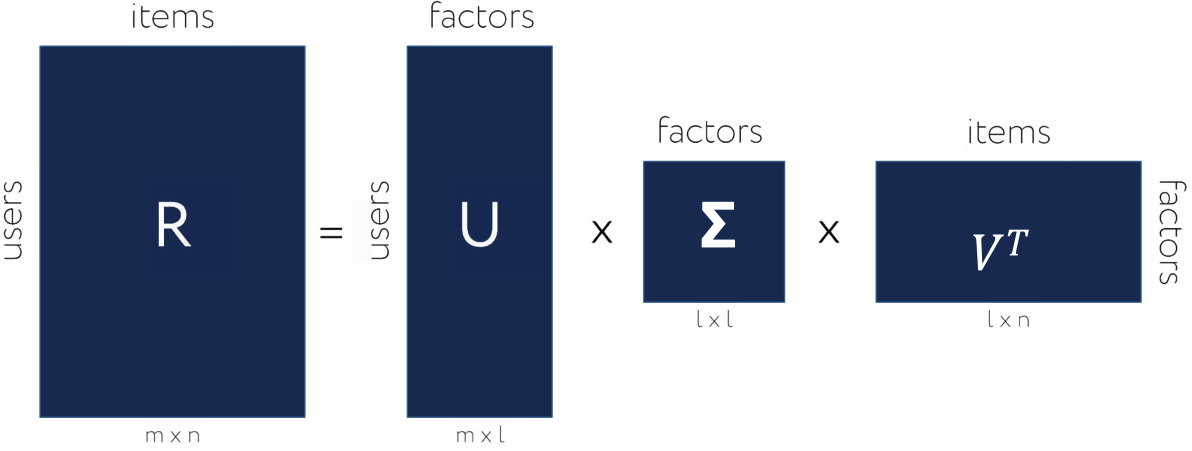
\includegraphics[height=0.35\textheight]{img/svd_user_item.png}
\end{center}
\end{frame}

\begin{frame}{SVD-разложение}
\begin{center}
    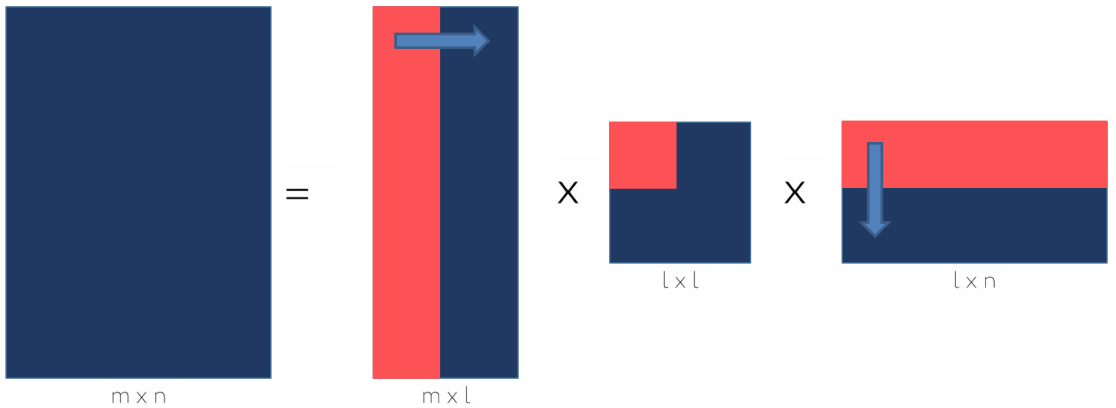
\includegraphics[height=0.35\textheight]{img/svd_user_item_1.png}
    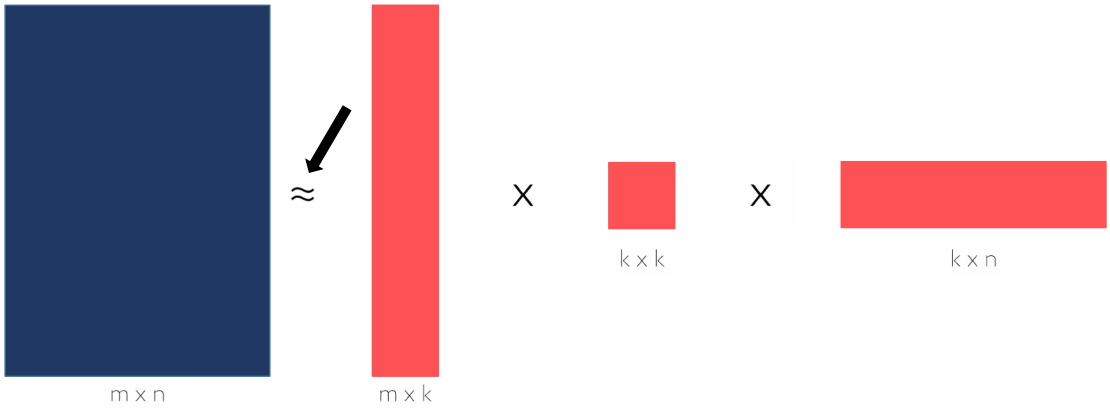
\includegraphics[height=0.35\textheight]{img/svd_user_item_2.png}
\end{center}
\end{frame}

\framedgraphic{Пример для рейтингов}{img/user_item_example.png}
\framedgraphic{Пример для рейтингов. SVD-разложение}{img/user_item_example_2.png}
\begin{frame}{Пример для рейтингов. Интерпретация.}
\begin{itemize}
    \item f1 -- энергичность,
    \item f2 -- "роковость", "брутальность\",
    \item f3 -- возможно, рандомный шум.
\end{itemize}
Оставим теперь две компоненты и посмотрим, насколько точно они приближают исходные значения.
\end{frame}

\begin{frame}{Пример для рейтингов. Точность приближения.}
\begin{center}
    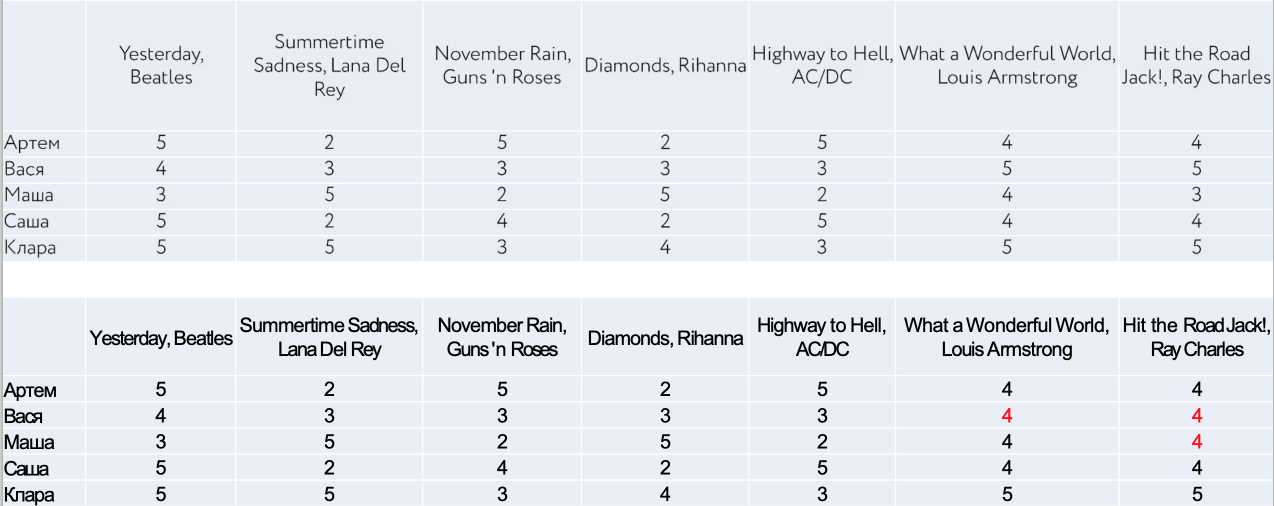
\includegraphics[width=\textwidth]{img/user_item_example_3.png}
\end{center}
Ошиблись только в трёх компонентах, и то чуть-чуть.
\end{frame}

\begin{frame}{Плюсы, минусы, подводные камни}
\begin{itemize}
    \item Позволяет сравнительно быстро строить рекомендации (по построенному SVD-разложению).
    \item Интерпретируемо. Позволяет понять, как устроены наши пользователи и объекты, имея информацию только о проставленных рейтингах.
    \item Матрица $R$ по-прежнему имеет дырки, и их нужно как-то заполнять.
    \item Само SVD-разложение строится долго для больших матриц.
    \item SVD-разложение не единственно.
\end{itemize}
\end{frame}

\section{Алгоритм Funk SVD}

\begin{frame}{Идея алгоритма}
\begin{itemize}
    \item Используем идею понижения размерности: пусть пользователи и объекты представляются как векторы $p_u$ и $q_i$ в некотором $k$-мерном пространстве. Тогда ищем предсказание рейтинга в виде $\hat r_{ui} = \langle p_u, q_i \rangle$.
    \item $\Theta = \{p_u, q_i\;|\; u\in U, i\in I\}$ – множество неизвестных параметров модели, которые нужно подобрать. Всего $(M+N)\cdot K$ параметров.
    \item Минимизируем квадратичное отклонение: $L = \sum(\hat r_{ui} - r_{ui})^2 \rightarrow \min_{\Theta}$.
    \item Если делать в лоб, то координаты $p_u$ и $q_i$ будут получаться очень большими. Поэтому лучше добавить ограничение на нормы $\|p_u\|$ и $\|q_i\|$. 
$$L(\Theta) = \sum_{(u, i)\in D}(\hat r_{ui} - r_{ui})^2  + \lambda \left(||p_u||^2 + ||q_i||^2\right) \rightarrow \min_{\Theta}.$$
    \item Суммируем только по известным рейтингам.
    \item Минимизируем через стохастический градиентный спуск.
\end{itemize}
\end{frame}

\begin{frame}{Алгоритм}
\begin{enumerate}
    \item Инициализируем матрицы $P_{N\times k}$ и $Q_{k\times M}$ (случайными числами).
    \item Пересчитываем $P$ и $Q$. Сдвигаемся по антиградиенту:
    $$P\;+= \alpha \cdot (\underbrace{E\cdot Q^T - \lambda P}_{\frac{\partial L}{\partial P}}), \;\;\;\;\;\; Q\;+= \alpha\cdot(\underbrace{E^T\cdot P - \lambda Q}_{\frac{\partial L}{\partial Q}}),$$
    где $E_{N\times M} = r_{ui} - \hat r_{ui}$, $\alpha$ -- learning rate -- параметр градиентного спуска.
    \item Повторяем п.2 до сходимости.
\end{enumerate}
Замечания:
\begin{itemize}
    \item Матрица $E$ содержит пропущенные значения, поэтому в матричных произведениях $EQ^T, E^TP$ суммировать нужно только по существующим значениям.
    \item Для ускорения расчётов произведений $EQ^T, E^TP$ можно на каждой итерации градиентного спуска оставлять только малую часть пар $(u, i)$. Это и является сутью стохастического градиентного спуска. Количество итераций до сходимости увеличится, но общая скорость сходимости для больших $N, M$ увеличится.
\end{itemize}
\end{frame}

\begin{frame}{Алгоритм Funk SVD}
\begin{itemize}
    \item Всё то же самое, только добавляем к предсказанию индивидуальные (константные) свойства пользователя $b_u$, объекта $b_i$ и среднее по датасету $\mu$:
    $\hat r_{ui} = \langle p_u, q_i \rangle + b_u + b_i + \mu$.
    \item Оптимизируем:
$$L(\Theta) = \underbrace{\sum_{(u, i)\in D}(\hat r_{ui} - r_{ui})^2  + \lambda \left(||p_u||^2 + ||q_i||^2 + b_u + b_i \right)}_{\rightarrow \min_{\Theta}}.$$
    \item Этот алгоритм занял третье место в Netflix prize (Simon Funk, 2006) и приобрёл большую популярность позже.
    \item Подобная техника применяется в нейронных сетях: трансформация объекта в произвольное $k$-мерное пространство называется embedding.
\end{itemize}
\end{frame}

\begin{frame}[allowframebreaks]
    \frametitle{Литература}
    \bibliographystyle{unsrt}
    \nocite{rec_systems_cs_center}
    \nocite{rec_systems_habr}
    \nocite{koren_recommender}
    \bibliography{references.bib}
\end{frame}

\end{document}